\documentclass[10pt,a4paper]{article}
\usepackage{tikz} % for drawing figures
\usepackage{amsmath} % for equations
\usepackage{url} % for URLs
\usepackage{graphicx}
\usepackage{multicol}
\usepackage{varwidth}
\usepackage{blindtext}


\usepackage{linguex} % ** special include in directory: for doing handy example labeling and bracketing
\renewcommand{\firstrefdash}{} % used for linguex package not to put hyphens in example refs (1a instead of 1-a)
%\usepackage{cogsci}
\usepackage{pslatex}
\usepackage{apacite}
\usepackage{placeins}

\newcommand{\sem}[1]{\mbox{$[\![$#1$]\!]$}}
\newcommand{\lam}{$\lambda$}
\newcommand{\gcs}[1]{\textcolor{blue}{[gcs: #1]}} 


% Possible title: Higher order pragmatic reasoning in reference games

%\title{On the purpose of ambiguous utterances}
\title{Social Learning via Ambiguity}
%\author{\large \textbf{our names}\\
%our emails\\
%our affiliations}


\begin{document}
\maketitle

\begin{abstract}
Seemingly in contradiction to Grice's maxim of manner, which postulates that ambiguity should be avoided during conversations to maximize clarity, ambiguity is ubiquitous during conversations.
Some ambiguity may be useful for efficiency reasons in cases when clarity is not affected.
Here we show that ambiguity can have another, socially highly relevant benefit: responses to ambiguous utterances reveal parts of the internal model of the interpreter.
We ran two main types of experiments online using a modified version of the original reference game experiment \cite{frankgoodman2012} and modeled the recorded response data by enhancing the Rational Speech Act framework.
We asked (i) whether speakers can use ambiguity resolving responses as a source of information about the unknown preferences of their conversation partner and (ii) whether speakers are able to strategically chose ambiguous over unambiguous utterances to learn about the preferences of their conversation partner.
The experimental and modeling results confirm both points. 
Participants were able to infer Bayesian posteriors of listeners' preferences when analyzing their choice of objects in a situation of referential ambiguity.
Moreover, in the second type of experiment, nearly 40\% of the speakers were able to strategically choose ambiguous over unambiguous utterances in an epistemic, goal-directed manner, maximizing expected information gain about the listener's preferences.
Surprisingly, an equally large number of participants seemed to minimize expected information gain by systematically choosing unambiguous utterances. 
Our results thus show that ambiguity resolution can reveal aspects of the knowledge, preferences, and beliefs of conversation partners and some of us are able to strategically use (ambiguous) utterances to gain knowledge about some of these aspects.
%We investigated and modeled how speakers learn about opinions, preferences, and beliefs of their conversation partners when monitoring their responses.
%Moreover, we asked the question whether 
%Accordingly, 
%The resulting model is additionally able to 
%(i) infer Bayesian posteriors of listeners' preferences when analyzing their choice responses to (ambiguous) utterances dependent on the number of options they have, and 
%(ii) choose (ambiguous) utterances by maximizing (or minimizing) expected information gain about the listeners preferences. 
%The modeling results show that 
%In this latter case, our model fits the participants' utterance choices revealing two main groups: while the one
%This group of speakers maximized expected social information gain (expecting to learn more about others). Another %group of participants seemed not interested in social learning, effectively minimizing the expected gain. 
%Overall, we essentially show that when monitoring a conversational partner's responses to our (partially ambiguous) utterances, we socially learn about the partner's inference model, revealing, for example, their preferences, opinions, and beliefs. 
%Moreover, some of us can choose utterances that are expected to yield the highest social information gain about (particular parts of) the partner's inference model.
%We discuss these situations of social learning in light of the predictive mind paradigm: we show how ambiguity in communication creates opportunities for conversation partners to build accurate predictive models of each other.                                                                    

\textbf{Keywords:} 
ambiguity; pragmatics; information gain; predictive priors; Rational Speech Act model
\end{abstract}

\section{Introduction}

The anticipatory nature of the human mind reveals itself in many domains.
We anticipate future events and event boundaries and pre-plan our hand movements even before we start moving \cite{Hayhoe:2004,belardinelli2016s, belardinelli2018mental, lohmann2019hands}, revealing anticipatory active inference processes in the sensory-motor domain.
In the language domain predictions span across a variety of tasks.
Listeners predict the semantic category of upcoming words \cite{federmeier2002picture} as evidenced by a neurophysiological effect known as N400.
Comprehension of sentences relies not only on the ability of listeners to anticipate subsequent words based on their transitional probabilities, but also takes into account the structural properties of sentences, revealing an even more abstract level of predictions \cite{levy2008expectation}.
Dynamic language models show that complex, event-predictive structures guide ambiguity resolution during comprehension and likely also constrain ambiguity generation during language production \cite{MyRaeElman:2019}. 

These processes have recently been linked to the predictive mind perspective \cite{Friston:2015,Hohwy:2013,Clark:2014}, proposing that our cognitive mind may be best characterized by an event-predictive inference system \cite{Butz:2016,Butz:2017}.
Various discipline associated with cognitive science provide evidence and theoretical considerations in this respect, including neuroscience, linguistics, developmental psychology, and philosophy \Cite{Zacks:2019,Baldwin:2019,...}.
The closely related, active inference mechanism \cite{PezzuloFristonSchwartenbeck:2016?} implies that our behavior is both, goal-directed and epistemic, expecting increases in internal homeostasis and knowledge gain, respectively.
Here, we reveal socially epistemic actions and interaction interpretations, gaining knowledge about the internal models, which are assumed to be used to interpret ambiguous utterances by the conversation partner.

In two main studies, we show how speakers update predictive models of the listener's preferences and beliefs when watching social event interactions, such as when offering a few entities to choose from and observing the choice of the partner. 
We thus show that humans can interpret behavior of other people as driven by their motives, intentions, or personal characteristics.
Conceptually, this idea goes back to the attribution theory \cite{jones1965acts, kelley1967attribution, kelley1970social}.
More recently, \citeA{shafto2012learning} developed a Bayesian model of learning that formalizes the process of inferring others' knowledge about the world based on their actions and goals. 

Here we focus on the situation of ambiguity resolution as a situation that lets the conversation partners observe each other's behavior and reason about internal beliefs that lead to particular choices of interpretations.
Moreover, we adapt the Rational Speech Act model framework, reliably modeling the involved, probabilistic interpretation processes as well as epistemic action choice. 
Interestingly, the modeling work reveals good interpretive abilities but also strong individual differences when the task is to choose (ambiguous) utterances strategically for gaining social knowledge. 


The rest of the paper is structured as follows: in Section 2 we first review how different disciplines approached ambiguity in natural language and communication, and then provide a computational background on referential ambiguity resolution. In Section 3, we develop models that are able to infer the preferences of the agent that led her to a particular choice of objects, as well as a model that predicts which utterances are most useful to create the possibility of learning. Sections 4 and 5 demonstrate the results of behavioral experiments, followed by a discussion in Section 6 where we conclude that participants in our experiments were indeed able to use observable behavior of others to infer their prior beliefs, and hypothesize why the ability to intentionally create situations leading to possible learning can be found only in a part of the population.

\section{Ambiguity in natural language and communication}
\subsection{Theoretical approaches}

If a speaker and a listener understand an ambiguous utterance differently, communication between them might fail. On rare occasions, such communication failure is deadly. \citeA{pinker2015sense} alludes to the Charge of the Light Brigade during the Crimean war as an example of a military disaster that was caused by vague orders. He also mentions how poor wording on a warning light was responsible for the nuclear meltdown at Three Mile Island. Finally, citing \citeA{cushing1994fatal}, Pinker describes how the deadliest plane crash in history resulted from pilots and air traffic controllers arriving at different interpretations of the phrase `at takeoff'.

Given that ambiguity can hinder the efficient transfer of information between conversation partners, it is not surprising that linguists have treated the possibility for ambiguity as a bug in the communication system \cite{grice1975,chomsky2002minimalism}. The attitude towards ambiguity has been quite different in other disciplines though, part of the reason being that the term itself can refer to multiple phenomena. For linguistic research, a word is ambiguous if it can have two separate meanings even in the absence of context, simply as a linguistic sign. In that sense, the word \textit{bat} is ambiguous between a winged mammal and sporting implement. In organizational communication, ambiguity aligns closely with underspecification: an utterance is ambiguous when it does not provide every detail about the intended interpretation, leaving room for the listener to interpret it. In the case of referential ambiguity, an ambiguous utterance may apply to several possible referents in a scene. For example, a pronoun can be referentially ambiguous if there are multiple potential antecedents in the context. It is the latter type that we will be concerned with in this paper.

If we look back at the study of ambiguity, we notice that the strategy of ambiguity avoidance is much older than the pronouncements of modern linguists. Greek and Latin rhetoricians believed that a skillfully written text allows for a perfectly accurate and lossless transmission of meaning to the listener or reader \cite{ossarichardson2019}; such a text avoids ambiguities.

Still, despite the teachings of classical philologists, authors continued to  create ambiguous texts and readers were faced with the challenge of interpreting them. The Bible is one of the most significant of such texts. In the sixteenth century, the Catholic church responded to the Reformation by proposing that the Bible can contain multiple meanings---\citeA{ossarichardson2019} equates these meanings with multiple paths that lead readers to God. In a sense, this proposal contained one of the first acknowledgments of the virtue of ambiguity, though with a  special caveat---only God could introduce ambiguity, humans should not. The search for efficient transmission of meaning that lasted over millenia rested on an important assumption: we communicate to transfer knowledge to our conversation partner. It is the efficiency of this transfer that many experiments were designed to evaluate. To be more precise, communication was considered efficient if a subject could follow instructions precisely. Yet, ordering actions and following instruction are probably not  the most common types of communicative acts \cite{foppa1995mutual} and information-seeking might not be the only communicative task we engage in \cite{markova1995preface}
% \gcs{not sure what is meant by this last bit}. 

More recent research has begun to take notice of the efficiency ambiguity affords us: by relying on context to fill in missing information, we can reuse lightweight bits of language rather than fully specifying the intended message \cite{levinson2000,piantadosietal2012,wasow2015}. 
Viewed in this way, ambiguity serves as a feature---not a bug---of an efficient communication system.
This reasoning accords with years of psycholinguistic research documenting that speakers readily produce ambiguous utterances (see \citeNP{ferreira2008}, for an overview). 
Along related lines, \citeA{wasow2015} reviews a large body of evidence and concludes that ambiguity is rarely avoided, even in situations where it would be communicatively appropriate.
This observation stands at odds with the Gricean maxim to avoid ambiguity (\citeNP{grice1975}).
However, even \citeauthor{grice1975} recognized a case of strategic ambiguity where it could be the intention of the speaker to communicate both possible interpretations afforded by an ambiguous utterance. In such cases, recognition of the ambiguity serves as the communicative purpose of the utterance. \citeauthor{wasow2015}, on the other hand, reviews several cases where ambiguous production serves no obvious communicative purpose.

The field of communication sciences views ambiguity as an important communicative tool. %\footnote{We would like to thank an anonymous reviewer at XPrag Conference for highliting the relevance of this field of study.} 
In organizational communication---communication that aids production---ambiguity has traditionally stood in opposition to clarity. However, as \citeA{eisenberg1984ambiguity} notes, clarity is not necessarily a communicative goal in all conversations. Speakers may prefer to remain ambiguous to leave room for the listener's perspective. This freedom is important in communication between managers and their employees, particularly when managers set goals that should stimulate rather than limit future creativity \cite{mohr1983implications}. Ambiguity allows for the expression of ideas that are true of a group of people. For example, consider company slogans or vision statements, where the language must be vague enough to allow every member of the audience to relate to a company's avowed aims \cite{carmon2013}. 
%\gcs{I think we should specify what we mean by ``ambiguity'' early on} Ambiguous descriptions also allow speakers to avoid conflict 
\cite{pascale1981art}: interlocutors often employ utterances that allow for a range of interpretations and do not enforce a particular viewpoint.

\citeA{eisenberg1984ambiguity} further specifies that ambiguity does not necessarily stand in opposition to clarity. In communication with close friends, for instance, interlocutors can use incomplete phrases or vague referential expressions and nevertheless resolve the ambiguity in accordance with the speaker's intention through the use of restricted codes---shared knowledge and beliefs. The participants may not even perceive the utterances as ambiguous in such situations. It is possible that the awareness of a shared code gives rise to the sense of within-group cohesion and social bond between group members. Thus, members of the same group sense a high level of mutual understanding.

\subsection{Computational modeling}

In search of the communicative purpose of ambiguous language, the current work identifies an additional benefit in using such language: the \emph{extra} information we gain from observing how our listeners resolve ambiguity.
We propose that language users learn about each other's private knowledge by observing how they resolve ambiguity. If language does not do the job of specifying the information necessary for full interpretation, then listeners are left to draw on their opinions, beliefs, and preferences to fill in the gaps; by observing how listeners fill those gaps in, speakers learn about the opinions, beliefs, and preferences of the listeners.
In a dynamic, naturalistic conversation, speakers can take turns choosing ambiguous statements in order to leave room for their parter to fill the missing information in, thereby revealing opinions, beliefs, and preferences. 


By way of illustration, take the scenario in Figure \ref{FG-ref-game}. Suppose a speaker produces the single-word utterance ``blue'' in an attempt to signal one of the objects to a listener. The utterance is referentially ambiguous; the listener can choose either the blue square or the blue circle. Suppose further that, upon hearing ``blue,'' the listener selects the blue circle. In observing this choice, the speaker learns something about the private thoughts of the listener: what made her select the blue circle instead of the blue square? Perhaps the circle is more salient to the listener, or the listener has a preference for circles, or the listener may believe that the speaker has a preference for circles; there may even be mutual agreement that circles are to be preferred when possible. Importantly, by observing how the listener resolves the ambiguity in reference, the speaker can learn something about the private thoughts of the listener. 

\begin{figure}
	\centering
	
\includegraphics[width=2in]{images/rsascene.eps}
	\caption{A simple reference game scenario from \protect\citeA{frankgoodman2012}. In the game, speakers choose a single-word utterance to signal one of the objects to a listener. In this scenario, the speaker chooses between the utterances ``blue,'' ``green,'' ``square,'' and ``circle.''}
	\label{FG-ref-game}
\end{figure}

However, accessing this added information requires the speaker to reason pragmatically about the pragmatic reasoning of the listener---a higher-order pragmatic reasoning, as it were. In order to select a referent, the listener must interpret the utterance. We follow \citeA{frankgoodman2012} in treating this interpretation process as active pragmatic, probabilistic reasoning: the listener interprets an utterance by reasoning about the process that generated it, namely the speaker, who selects an utterance by reasoning about how a listener would interpret it. \citeauthor{frankgoodman2012} model this recursive social reasoning between speakers and listeners within the Rational Speech Act (RSA) modeling framework (for more on RSA as a framework, see also \citeNP{frankejaeger2016,goodmanfrank2016}).

The current paper builds on the foundational, vanilla RSA model of reference games by introducing uncertainty about the prior beliefs of the listener and modeling a speaker who reasons about these beliefs on the basis of and in anticipation of the observed referent choice. 
We begin by walking through our modeling assumptions. 
We then present our models in full detail, and test the behavioral predictions of our models against human data in a series of web-based experiments.
We conclude with a discussion of the significance of our findings for understanding ambiguity in natural language, and relate the findings to current theories of predictive coding and active inference.


\section{Model}
\subsection{Full pragmatic model}

We begin with the vanilla RSA model of \citeA{frankgoodman2012}. The recursive social reasoning inherent to the RSA modeling framework gets cashed out as various layers of inference. At the base, there is a hypothetical, na\"ive literal listener $L_0$ who hears an utterance $u$ and infers the state of the world $s$ that $u$ is meant to describe; that is, the object referred to by the utterance. $L_0$ performs this inference by conditioning on the literal semantics of $u$, \sem{$u$}. $L_0$ thus returns a uniform distribution over those states $s$ that can be truthfully described by $u$:
$$P_{L_{0}}(s\mid u) \propto \sem{$u$}(s).$$
One layer up, the speaker $S_1$ observes some state $s$ and chooses an utterance $u$ to communicate that state to $L_0$. $S_1$ chooses utterances on the basis of their utility for signaling $s$ to $L_0$, $U_{S_1}(u;s)$. The speaker's utility maximizes the probability that $L_0$ would arrive at the correct $s$ on the basis of $u$, $P_{L_{0}}(s\mid u)$\footnote{The original model in \citeA{frankgoodman2012} also includes a term for the cost of utterance $C(u)$. We eliminate the term here since we assume a uniform cost for all the utterances.}:
$$U_{S_{1}}(u;s) = \textrm{log}(P_{L_{0}}(s\mid u)).$$ 
$S_1$ chooses utterances in proportion to their utility:
$$P_{S_{1}} (u\mid s) \propto   \textrm{exp}(\alpha \cdot U_{S_{1}} (u;s)).$$
At the top layer of inference, the \emph{pragmatic} listener $L_1$ infers $s$ on the basis of some observed $u$. The result is a distribution over likely states $s$; however, unlike $L_0$, $L_1$ updates beliefs about the world by reasoning about the process that \emph{generated} $u$, namely $S_1$. In other words, $L_1$ reasons about the $s$ that would have been most likely to lead $S_1$ to choose the $u$ that was observed:
$$P_{L_{1}}(s\mid u) \propto P_{S_{1}}(u\mid s) \cdot P(s).$$

\citeA{frankgoodman2012} tested the predictions of their model against behavioral data from reference games, as in Figure \ref{FG-ref-game}. To model production behavior (i.e., which utterance should be chosen to communicate a given object), the authors generate predictions from $S_1$. To model interpretation behavior (i.e., which object the speaker is trying to communicate on the basis of their utterance), the authors generate predictions from $L_1$. Finding extremely high correlations between model predictions and behavioral data in both cases, \citeauthor{frankgoodman2012} have strong support for their model of pragmatic reasoning in reference games (see also \citeNP{qingfranke2015}, for a fuller exploration of the modeling choices).

Our model builds on the vanilla version of RSA presented above by allowing for uncertainty around the listener's state prior, $P(s)$. %In that sense, the model belongs to the family of models known as uncertain RSA \cite{goodmanfrank2016}. 
We have in mind a scenario where a listener might have a preference for a certain object feature (e.g., blue things, squares, circles, etc.), and these preference will influence their object choice. With this in mind, a pragmatic speaker produces an utterance $u$, observes the listener's referent choice $s$, and, on the basis of that choice, infers the preferences $f$ the listener might have had when making the choice.
We use the same $L_0$ and $S_1$ from the vanilla model. However, we now parameterize $L_1$'s state prior so that it operates with respect to a given feature preference $P(s\mid f)$:
$$P_{L_{1}}(s\mid u,f) \propto P_{S_{1}}(u\mid s) \cdot P(s\mid f).$$
We then model a pragmatic speaker $S_2$ who updates beliefs about $L_1$'s preferences, $P(f)$. To do so, $S_2$ produces $u$ and observes $L_1$'s choice of $s$, then reasons about the likely feature preference $f$ that $L_1$ used to make that choice:
$$P_{S_{2}}(f\mid u,s) \propto P_{L_{1}}(s\mid u,f) \cdot P(f).$$

We also model the reasoning process by which a speaker may select the best utterance to learn about the preferences of the listener.
Starting with no knowledge of the listener's preferences, $S_2$ can be assumed to expect a uniform (i.e., flat) feature preference prior $P(f)$. The more the speaker's posterior beliefs about the preferences, $P_{S_{2}}(f\mid u,s)$, deviate from the uniform prior, the more the speaker will have learned about the listener's preferences. 
We can thus model this reasoning in the light of expected information gain, which can be equated with the attempt to maximize the KL divergence between the speaker's flat prior and the expected posterior of the listener's feature preferences $f$, integrating over all hypothetically possible state observations $s$: %\gcs{can we assume a uniform cost and then remove $C(u)$ from our equations, mentioning this move in a footnote?}
$$P_{b}(u) \propto \sum_{s:\  [\![u]\!](s)}\lambda \cdot \textrm{KL}(P(f),P_{S_{2}}(f\mid u,s)).$$

We now have two sets of predictions from our model to check: first, the pragmatic speaker's inference about the listener's feature preferences on the basis of their object choice; and second, the pragmatic speaker's strategic utterance selection in the light of the anticipated information gain about the listener's preferences considering their possible object choices. Below, we present two experiments that test these predictions against human behavior.

\subsection{Simplified pragmatic model}

\citeA{sikos2019} demonstrate that simpler models with fewer layers of reasoning perform as well or better than more complex models in simple reference games. In fact, their simplified model with only an enhanced $L_0$ equipped with an informative prior outperformed the full vanilla RSA model when it came to predicting interpretation behavior, suggesting that participants engage in shallower reasoning than predicted by the full-blown RSA. We therefore compare the predictions of our full pragmatic model with those of a simplified model model.

Our simplified model involves an enhanced literal listener that updates the preference-specific state prior $P(s\mid f)$:
$$P_{L_{0\textrm{-simp}}}(s\mid u,f) \propto \sem{$u$}(s) \cdot P(s\mid f).$$
In the simplified model, the pragmatic speaker $S_{1\textrm{-simp}}$ reasons directly about the enhanced $L_{0\textrm{-simp}}$, rather than about $L_1$ who in turn reasons about $S_1$'s reasoning about $L_0$.

$$P_{S_{1\textrm{-simp}}}(f\mid u,s) \propto P_{L_{0\textrm{-simp}}}(s\mid u,f) \cdot P(f).$$


\section{Experiment 1: Inferring preferences}

Our first task is to check the predictions of our pragmatic speaker layer: having observed that a listener selects some object $s$ in response to an utterance $u$, what are the most likely preferences the listener had when making their choice? 

\subsection{Participants}

We recruited 90 participants with US IP addresses through Amazon.com's Mechanical Turk crowdsourcing service. Participants were compensated for their participation. On the basis of a post-test demographics questionnaire, we identified 82 participants as native speakers of English; their data were included in the analyses reported below.

\subsection{Design and methods}

We presented participants with a series of reference game scenarios modeled after Figure \ref{FG-ref-game} from \citeA{frankgoodman2012}. Each scenario featured two people and three objects. One of the people served as the speaker, and the other served as the listener. The speaker asks the listener to choose one of the objects, but in doing so she is allowed to mention only one of the features of the target object. Participants were told that the listener might have a preference for certain object features, and participants were tasked with inferring those preferences after observing the speaker's utterance and listener's object choice.

We followed \citeA{frankgoodman2012} in our stimuli creation. Objects were allowed to vary along three dimensions: color (blue, red, green), shape (cloud, circle, or square), and pattern (solid, striped, polka-dotted). The speaker's utterance was chosen at random from the properties of the three objects present, and the listener's choice was chosen at random from the subset of the three objects that possesed the uttered feature. By varying the object properties, the targeted object, and the utterance, we generated a total of 2400 scenes. Speaker and listener names were chosen randomly in each trial. Participants saw the speaker's utterance in bold (e.g., ``red'' in Figure \ref{exp1-trial}) and the listener's choice appeared with a dotted orange outline (e.g., the center object in Figure \ref{exp1-trial}). Based on the observed choice, participants were instructed to adjust a series of six sliders to indicate how likely it is that the listener had a preference for a given feature. The sliders specified the six feature values of the two feature dimensions that were not mentioned in the speaker's utterance (e.g., pattern and shape in Figure \ref{exp1-trial}). 

Depending on how many features objects share with the target object (marked by a frame in each trial), we were able to identify 48 ambiguity classes. Ambiguity classes group trials where a model considers a similar number of alternatives that could qualify for the uttered feature. For example, in Figure \ref{exp1-trial}, the utterance \textit{red} picks out 2 possible objects. If, however, the utterance was \textit{green}, only 1 object would qualify, and no learning about preferencs would be possible. In that case, the model would assign equal probability that a person likes dotted objects, striped objects, clouds, or squares. Once the model establishes that more than 1 object can be picked, it also needs to consider whether alternative objects share their features with the target object. For example, if both red objects were also striped, the model would not be able to infer any preferences about the pattern. Finally, we also code whether the objects that were not picked are similar in any of their feature values.

Participants completed a series of $15$ trials. Objects and utterances were chosen as detailed above, with the constraint that 10 trials were potentially informative with respect to listener preferences and 5 trials were uninformative with respect to listener preferences (e.g., observing that the listener chose one of three identical objects). 

\begin{figure*}[ht!]
	\centering
	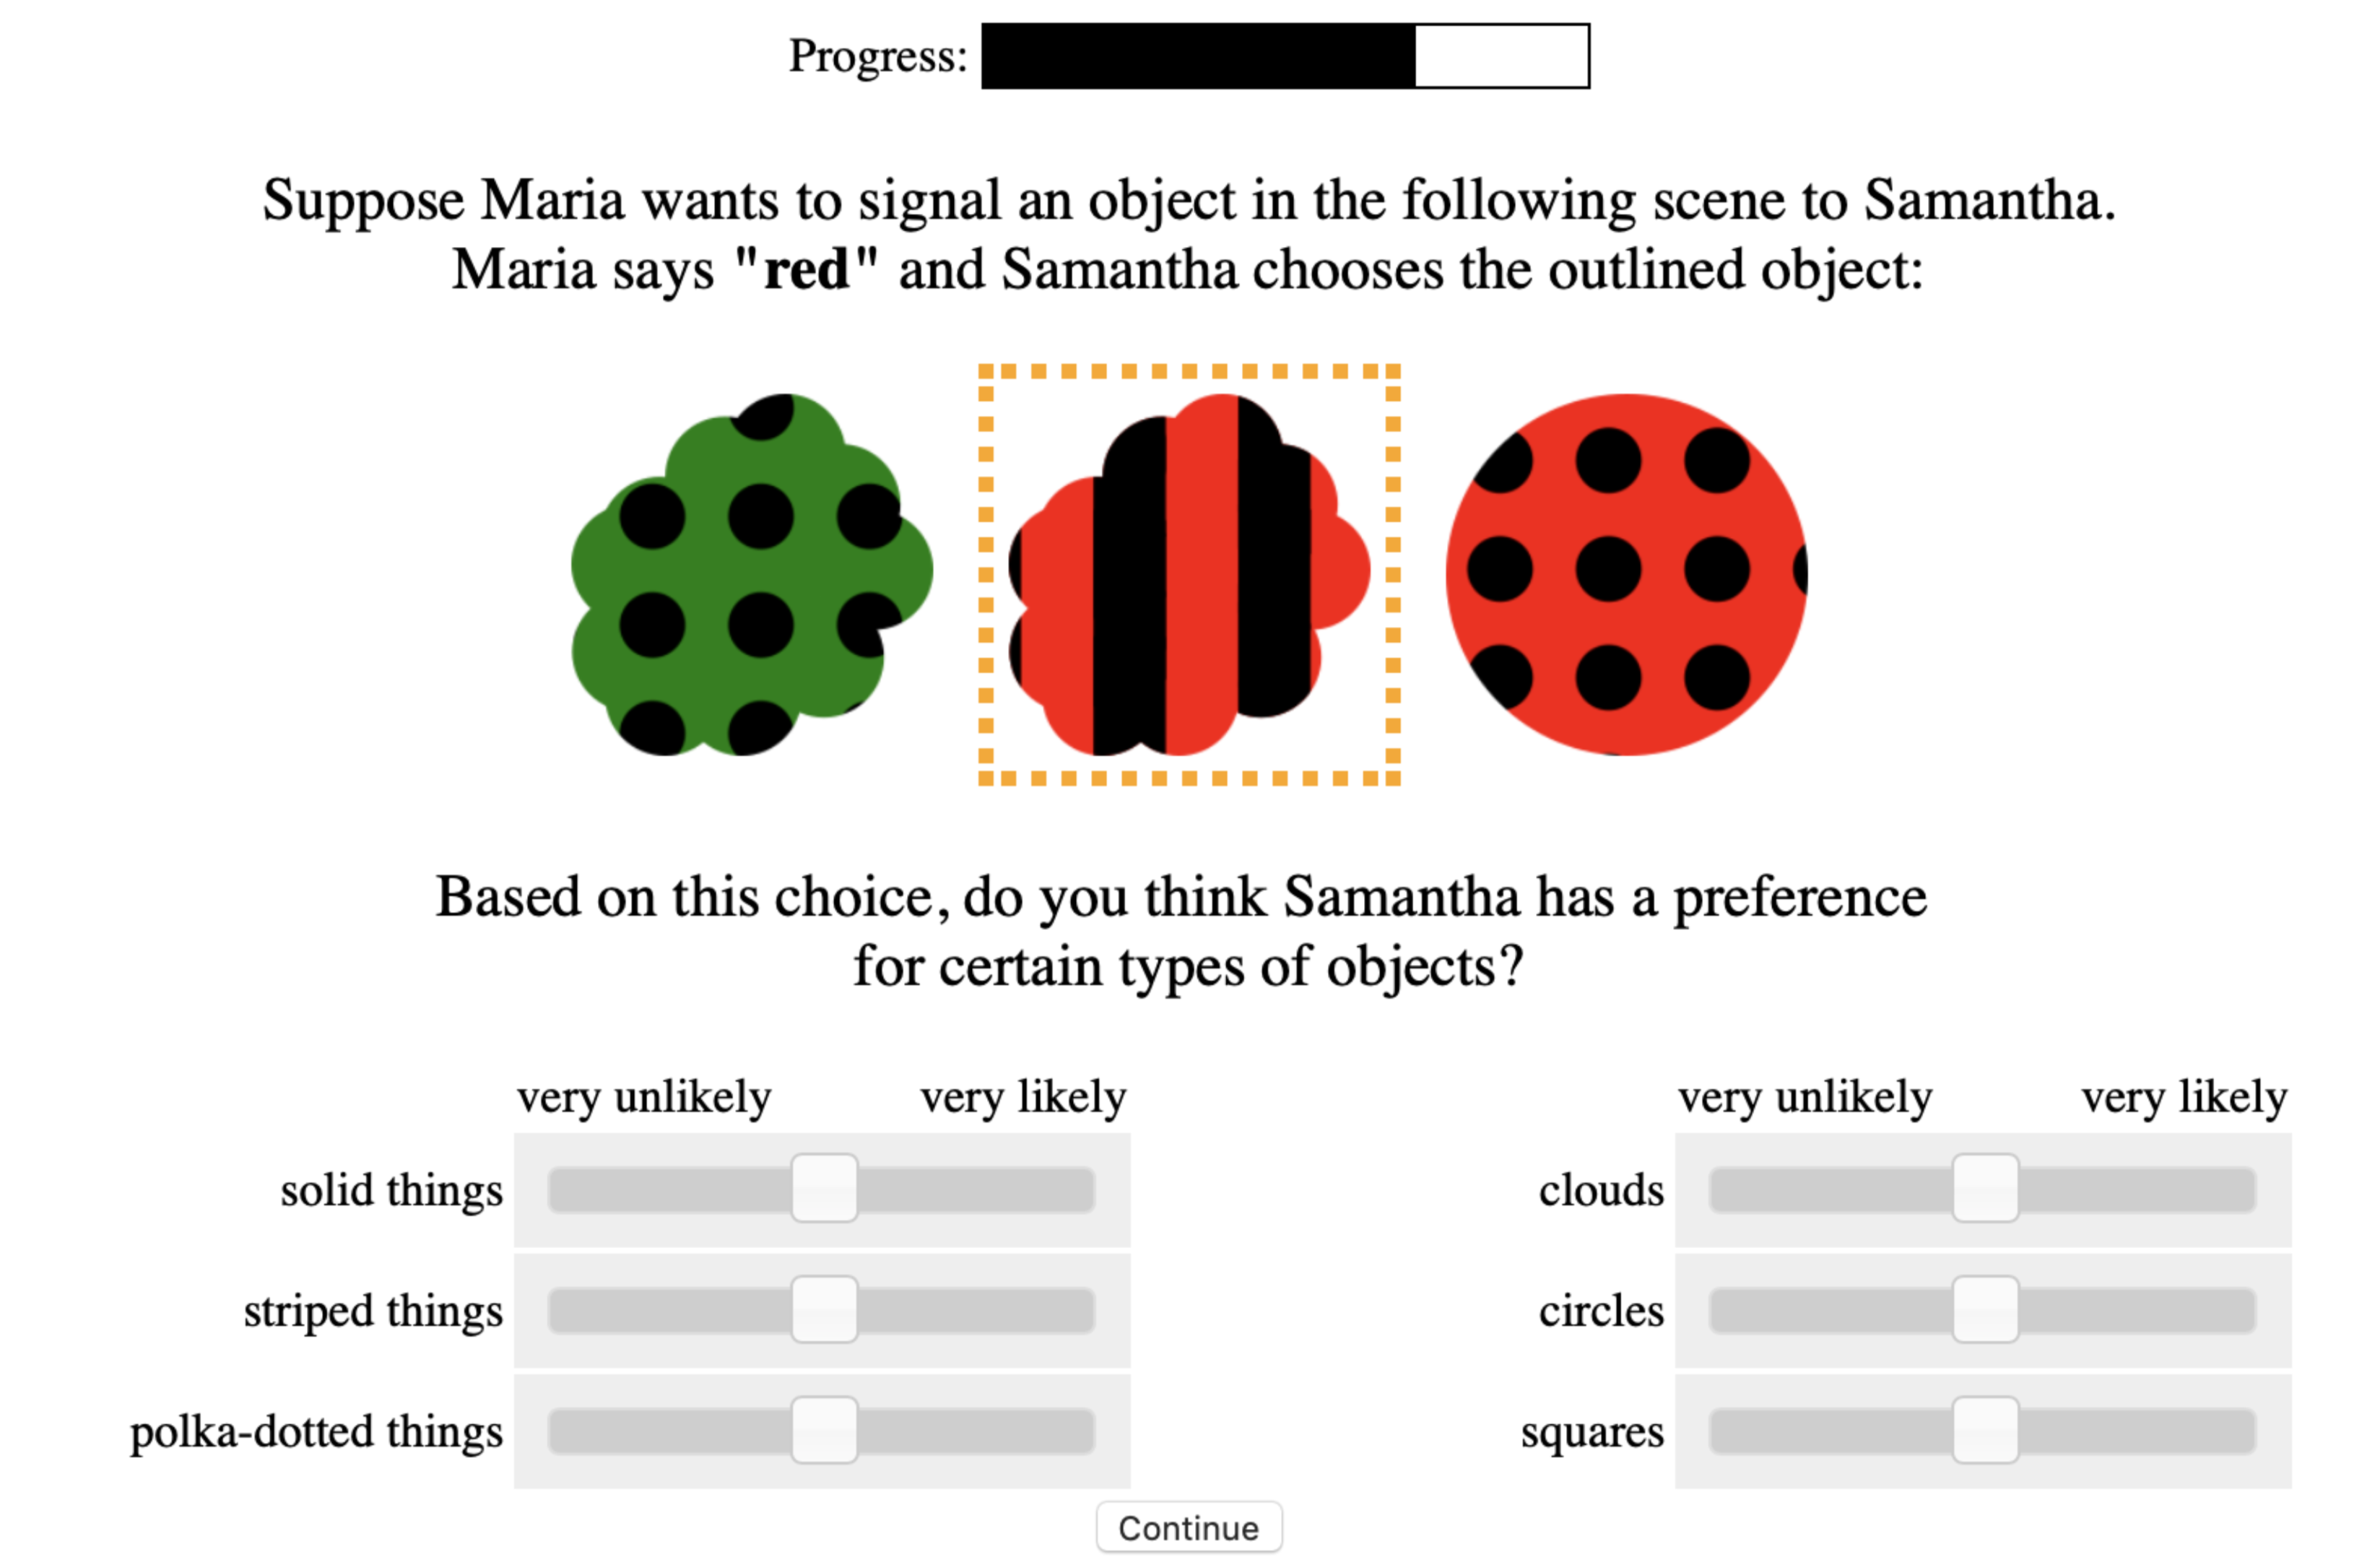
\includegraphics[width=4.5in]{images/preference-trial.png}
	\caption{A sample trial from \emph{Experiment 1: Inferring preferences}.}\label{exp1-trial}
\end{figure*}

\subsection{Results}

\subsubsection{Models with global optimization}

To compare RSA model predictions to the human data, we calculated an average value for each slider binning data into 48 ambiguity classes. We excluded the sliders if their corresponding feature value as not present in a scene. For example, for Figure \ref{exp1-trial} we excluded the sliders for solid things and squares since none of these are present, and therefore no learning is possible.
%We binned those scene types 
%For all scene types, the actual feature values and objects in a scene were reordered according to the specific preference inference involved \gcs{I'm not sure what you mean here}. 
%Thus, after reordering, the results of the individual slider values for individual scenes in each scene type could be averaged for both the participant data and the model predictions. 

We performed two types of optimization: at the individual level and at the global group levels by optimizing a Kullback-Leibler divergence between the data and the model predictions:

$$\textrm{KL} = \sum_{i=1}^{n} P(f'_i\mid u,s) (\textrm {log} (P(f'_i\mid u,s) - \textrm {log} (P(f_i\mid u,s)),$$

where $P(f'_i\mid u,s)$ specifies a participant's normalized slider value settings, which offer empirical estimates of the feature preference posterior given an object scene and a particular utterance $u$ and object choice $s$; $P(f_i\mid u,s)$ specifies the respective model prediction value. 
Since no conclusions can be drawn concerning feature values that are not present in the scene, we ignored the respective feature preference estimates. By minimizing KL divergence between the empirical and model-predicted preferences for each participant, we maximize the model fit to the individual participants' data. We can then use the KL divergence values to perform the likelihood ratio test for nested models relying on the $G^2$-statistic which is approximately chi-square distributed \cite{Lewandowsky:2011}. 

We first present the globally-optimized versions of the model (Figure \ref{simple-full}). We fit three parameters for the full RSA model, and two for the simple model. We hypothesized that participants may either go through all the layers of pragmatic reasoning, and additionally calculate the preferences that lead to particular object choice. The last layer of this model $S_2$  returns a posterior distribution over inferred feature preferences $f$ after observing a listener selecting an object in response to an utterance. In a simpler model, the object choice is driven only by a $L_0$ semantics enhanced with priors over feature preferences. Upon hearing an utterance \textit{blue} a participants assigns equal probabilities to all blue objects in a scene, and the actual choice of object signals a preference of other feature values that object has. For example, picking a blue circle rather than a blue square is driven by a prefrence for circles.

For the full RSA model, the first parameter is the soft-max scaling factor $\alpha$ in the $S_1$ layer of the model, where the default value is typically set to $\alpha=1$ (i.e., no scaling). 
This parameter controls how likely $S_1$ is to maximize utility when choosing utterances. The simple model does not rely on this parameter.

The second parameter scales the softness of individual feature preferences $f_i$. This parameter controls the shape of each of the possible feature preferences $f_i$ that $S_2$ considers. 

$$ P(s\mid f) = \frac{P(s\mid f) + \gamma}{\sum P(s\mid f) + 3\gamma}$$
% I tried to write it in a more general form that works for both P = 0 and P = 1 but I'm not sure that works.
% This is the R code:
%objectPreferenceSoftPriors[[utt]] <- objectPreferenceHardPriors[[utt]] + softAddProb
%objectPreferenceSoftPriors[[utt]] <- objectPreferenceSoftPriors[[utt]] / sum(objectPreferenceSoftPriors[[utt]])
 %$$ P(s_{\textrm{cloud}}\mid f_{\textrm{cloud}}) = \frac{1 + \gamma}{1 + 3\gamma}$$
 % This is what we wrote. It makes sense for P = 1 but I'm not sure the numbers come out right when we calculate how softness changes the probability of objects that don't qualify.
 For example, in trial shown in Figure \ref{exp1-trial}, there are two objects that fit the description \textit{red}: a red striped cloud and a red dotted circle. The softness parameter $\gamma$ regulates the probability that the middle object will be picked if a person has a preference for clouds. Preference softness increases with $\gamma$: 
 a value of $\gamma=0$ specifies a hard preference, which means that the listener will always choose the object that holds the preferred feature value if possible (e.g., clouds when clouds are preferred). 
 We assume $\gamma=0$ as the default model value. Let us see how the probability changes if $\gamma$ is set to 0.2:
 
 $$ P(s_{\textrm{cloud}}\mid f_{\textrm{cloud}}) = \frac{1 + 0.2}{1 + 3 \cdot 0.2} = 0.75$$
 Here the preference becomes softer: a subject will pick up clouds with a probability of 0.75 rather than 1.
 On the other hand, $\gamma \rightarrow \infty$ specifies a uniform feature value preference, or no actual preference. As a result, a large value of $\gamma$ approximates a uniform-prior model.

%The softness parameter $\gamma$ determines how strong a preference is if a certain feature value is indeed preferred.
 %such that the RSA models can be viewed as being nested within the default model.
% Note: I removed $\beta$ because it complicates things enormously and proved to be not really relevant.

Finally, we allow for the possibility of noise in our human data introduced by participants not following instructions. The parameter $\beta$, when above 0, allows subjects to consider objects that do not pass the semantic filter of the literal listener. 

$$ P(s_{\textrm{x}}\mid u_{\textrm{x}}) = \frac{P(s\mid u) + \beta}{\sum P(s\mid u) + 3\beta}$$
As $\beta$ increases, speakers disregard instructions and assign non-zero probabilities to objects that do not correspond to the utterance; with $\beta = 0$, speakers fully obey the instructions and only consider objects with the named property (e.g., only red objects following the utterance \textit{red}).


Figure \ref{barplot_x4} presents the model performance for the scene type of the sample trial from Figure \ref{exp1-trial}. In that trial, participants saw that the middle object was chosen following the utterance \textit{red}. There are two potential referents for this description: a red striped cloud and a red dotted circle. Since the cloud was chosen, we infer that the person who chose this object has a preference for clouds over circles, and for striped objects vs.~dotted ones. From this trial, we cannot learn anything about the preference for solid things or squares, so we expect the subjects to leave the sliders in their default location (i.e., centered).
The barplot in Figure \ref{barplot_x4} shows that indeed when faced with a combination of objects from Figure \ref{exp1-trial}, both humans and the models assign high slider values to clouds and striped things, and low values of the sliders to circles and dotted things. In this plot we show two types of models: an optimized and a non-optimized one.

\begin{figure}[ht!]
	\centering
	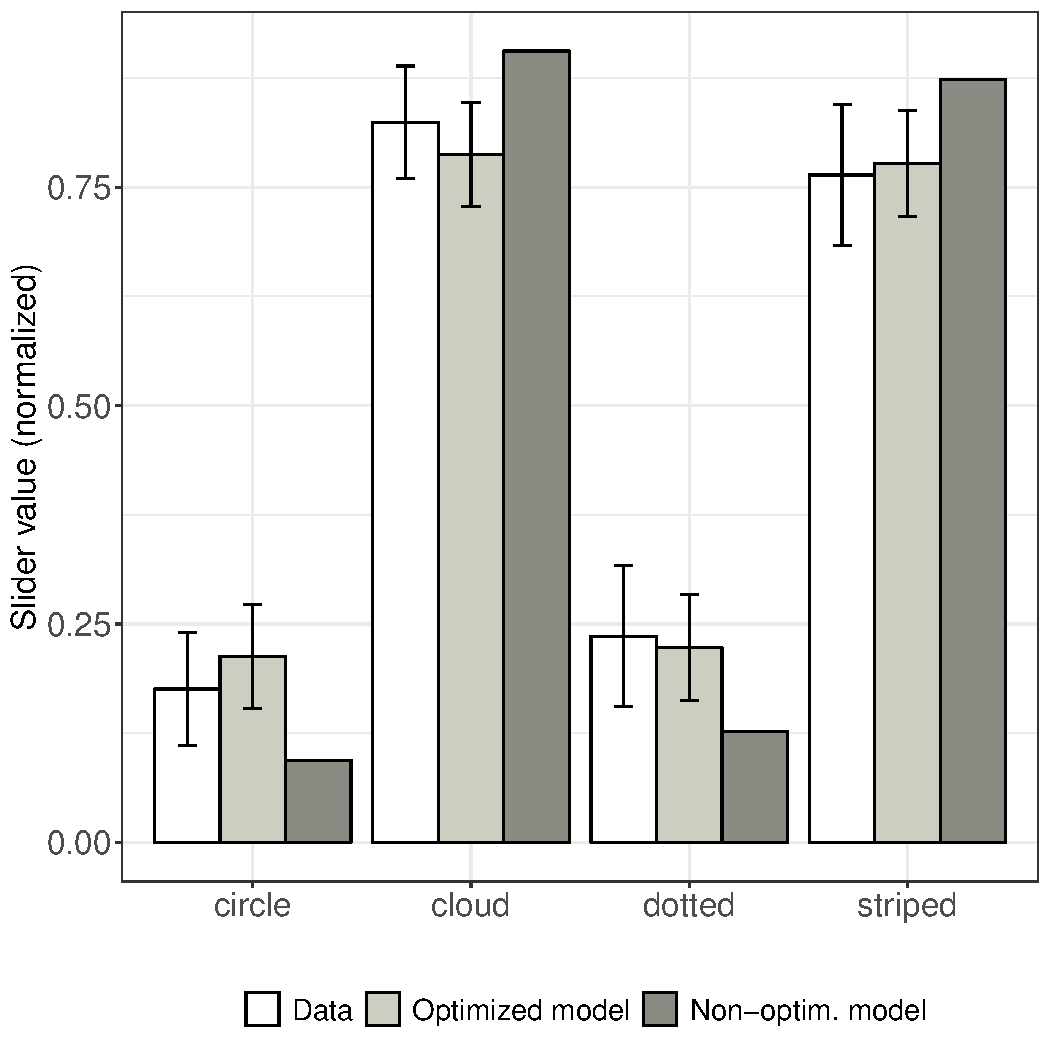
\includegraphics[width=2.5in]{images/barplot_x4.pdf}
	\caption{Model predictions and human data for one of the classes of stimuli \emph{Experiment 1: Inferring preferences}.}\label{barplot_x4}
\end{figure}

% I used the code length(levels(as.factor(uniqueCCode))) to calculate the number of conditions
%Since not all of the stimuli allowed for inference of preferences in the same way, we introduced a new categorization of stimuli. Our base model would then predict the same preferences for the same category of stimuli. The categorization takes into account the distribution of features, the chosen object and which feature was uttered. Each category consists of 3 tuples of 2 digits. Each tuple refers to one feature, where the first tuple always refers to the uttered feature. The first digit in each tuple would then denote how many objects share the value of the picked object for the corresponding feature. In figure \ref{FG-ref-game}, if the utterance was blue and the blue square was picked, the first tuple would reference color and its first digit would be a "2". Note that this does not determine which other object shares the feature value, i.e. "blue". To compensate, the second digit of the tuple denotes which other object shares this value. This depends on the order of the objects---we stipulated that the picked object would be the first. The further order would be determined by which other object shares this specific value, i.e. the "blue circle" in figure \ref{FG-ref-game} would be the first of the "other objects" and the "green square" the second. The picked object is at position zero in this sense. Thus the first tuple for figure \ref{FG-ref-game} would be (2,1). For the other tuples, the first digits would be "2" for shape and "3" for texture. To streamline the category code we stipulated that we would order the features in descending order of their first digit, so that we would have texture's "3" next in figure \ref{FG-ref-game}. If a tuple starts with "3" or "1", the second digit would simply denote whether the other objects have different values for that feature or the same. Thus we would have (3,2) for texture, with the second digit signaling that the non-picked objects share their texture. The tuple for shape would finally be (2,2), because the value "square" is shared with the second other object (see above). Thus for figure \ref{FG-ref-game} we would end up with [(2,1),(3,2),(2,2)].


Both, the simple and the full models with softness optimized globally provide a good linear fit to the data (simple model: $p < 0.001$, $r^2 = 0.86$; full model: $p < 0.001$, $r^2 = 0.86$) suggesting that participants are indeed able to infer the feature preferences that lead to a choice of an object. %We can also see that the simple model fits the data just as well as the full more complex model.

\begin{figure}[ht]
	\centering
	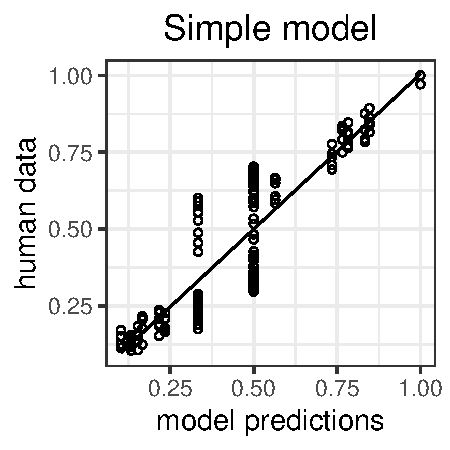
\includegraphics[width=2in]{images/m13.pdf}
	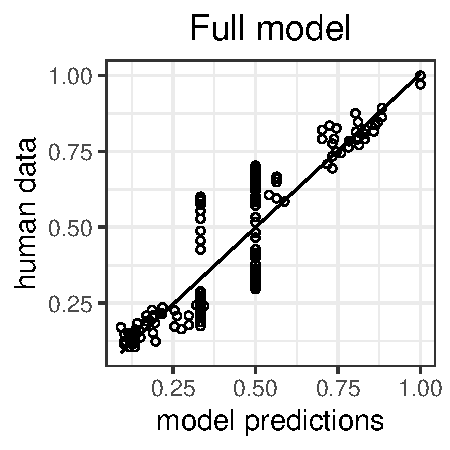
\includegraphics[width=2in]{images/m23.pdf}
	\caption{Average human data from Experiment 1 plotted against the predictions of the $\beta$-optimized RSA model; both models $r^{2}=0.86$, 95\% CI [0.80 0.90].}\label{simple-full}
\end{figure}

%\gcs{how was the fitting performed?}

\subsubsection{Individually-fitted models}

Model fit improves when we fit the parameters at the individual level, calculating a parameter estimate for each participant. Individual-level modeling allows us to explore potential differences between participants, and, more importantly, to evaluate whether the Gricean reasoning strategies apply at the level of individual speakers or only to population as a whole \cite{franke2016reasoning}. 

We optimized $\alpha$ and $\gamma$ in light of the KL divergence between the individual participants' slider value choices and the corresponding model predictions.



%the For example, if a $S_2$ observes that following an utterance $blue$ and three objects all three of which are blue, but all differ in shape, the speaker chooses a square, the speaker might conclude that the $L_1$  has a preference for squares. However, the exact value on the slider the $S_2$ picks depends on the $\gamma$ parameter: if it is close to $0$, the speaker will mark that the $L_1$ had a perefernce for squares close to $1$. As the parameter value increases, the softness of preference will increase as well, drawing the preference value towards uniform (uninformative).
%he model contains three parameters: the informativity paramter $\alpha$ (how informative speakers choose to be), the obey-instructions parameter $\beta$, and the softness of preferences parameter $\gamma$. The latter 

% \gcs{We need to say something about how we fit individual participant data. How exactly where the parameter values fit? What were candidate values?}



\begin{figure}[ht]
	\centering
	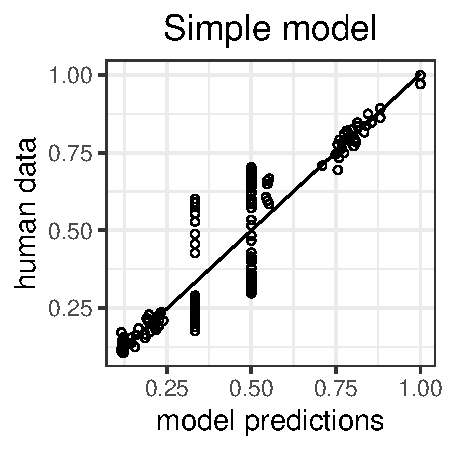
\includegraphics[width=2in]{images/m3.pdf}
	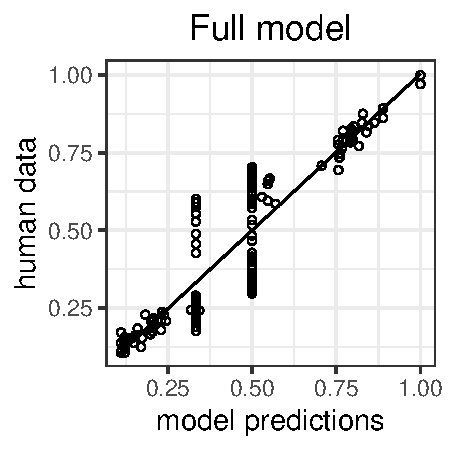
\includegraphics[width=2in]{images/m16.pdf}
	\caption{Average human data from Experiment 1 plotted against the predictions of the individually $\gamma$-optimized simplified RSA model $r^{2}=0.86$, 95\% CI [0.81 0.90] and $\gamma$ and $\alpha$ optimized full RSA model; $r^{2}=0.86$, 95\% CI [0.80 0.90].}\label{simple-full-individual}
\end{figure}

Figure \ref{simple-full-individual} demonstrates that the full model optimized at the individual level for an additional parameter $\alpha$ does not improve the fit compared to the simplified model. Since the two models account for the same amount of variance in the data, we will proceed with the simplified model evaluation.



%When compared to the uniform-distribution base model, optimizing $\gamma$ alone yielded a much lower KL divergence value: while the uniform base model yields an average KL divergence of $9.848$ (median=$7.028$), our extended RSA model with individually-optimized $\gamma$ parameters yielded an average KL divergence of $2.058$ (median=$1.524$). 
%When optimizing $\alpha$ and $\gamma$ together, a yet smaller average KL divergence of $1.451$ (median=$0.952$) is reached.
%In the light of the $G^2$ statistics and under the assumption that we calculated $2$ KL divergences in all $15$ trials per participant, the KL values should be multiplied by $2*15*2=60$ to yield a $G^2$ estimate, although one may want to consider the two KL divergences in each trial as closely related, such that $2*15=30$ may be considered as a more passive multiplier.


%With this factor, we get a difference of $233.7$ between the uniform base model and the one-parameter extended RSA model, while the additional optimization of $\alpha$ improves $G^2$ further by a value of $18.21$. Both of these results are far above the cutoff value of $6.63$ for $p=.01$, assuming a Chi-square distribution \cite{Lewandowsky:2011}. 
%Thus, the extended model exceeds the uniform base model with very high likelihood. 
%However, considering the much smaller improvement due to the additional optimization of $\alpha$, we analyze correlations with respect to the one-parameter (i.e., $\gamma$-optimized) model in what follows. 

%When considering the distribution of optimized parameters, we can identify three participants who cause the optimization process to yield $\gamma$ values above $100$, indicating lazy participants who simply leave the slider values unadjusted. 
%Another 15 participants yielded a $\gamma$ value above $1$, which indicates that they are considering preferences only to a small extent. The rest (i.e., 64 participants) yielded values below $1$, indicating a strong consideration of preference inferences in line with the model. 
 
%We compared  in the light of the distinguishable interpretation cases. 

We plot predictions from the $\beta$ and $\gamma$-optimized model in Figure \ref{cross-validation}, where a strong positive correlation between the human judgments and model predictions ($r^2 = 0.99, p < 0.001$) can be observed. The likelihood ratio test revealed that a $\gamma$ and $\beta$-optimized model provides a better fit compared to a model optimized only for $\gamma$ ($G^2 = 237.36, df = 82, p < 0.01$). The more complex model contains one additional parameter $\beta$ fitted for each subject giving us 82 degrees of freedom. We additionally check the generalizability of the model by performing a leave-one-out cross-validation. We show in Figure \ref{cross-validation} that the cross-validated model retains its fit.

\begin{figure}[ht]
	\centering
	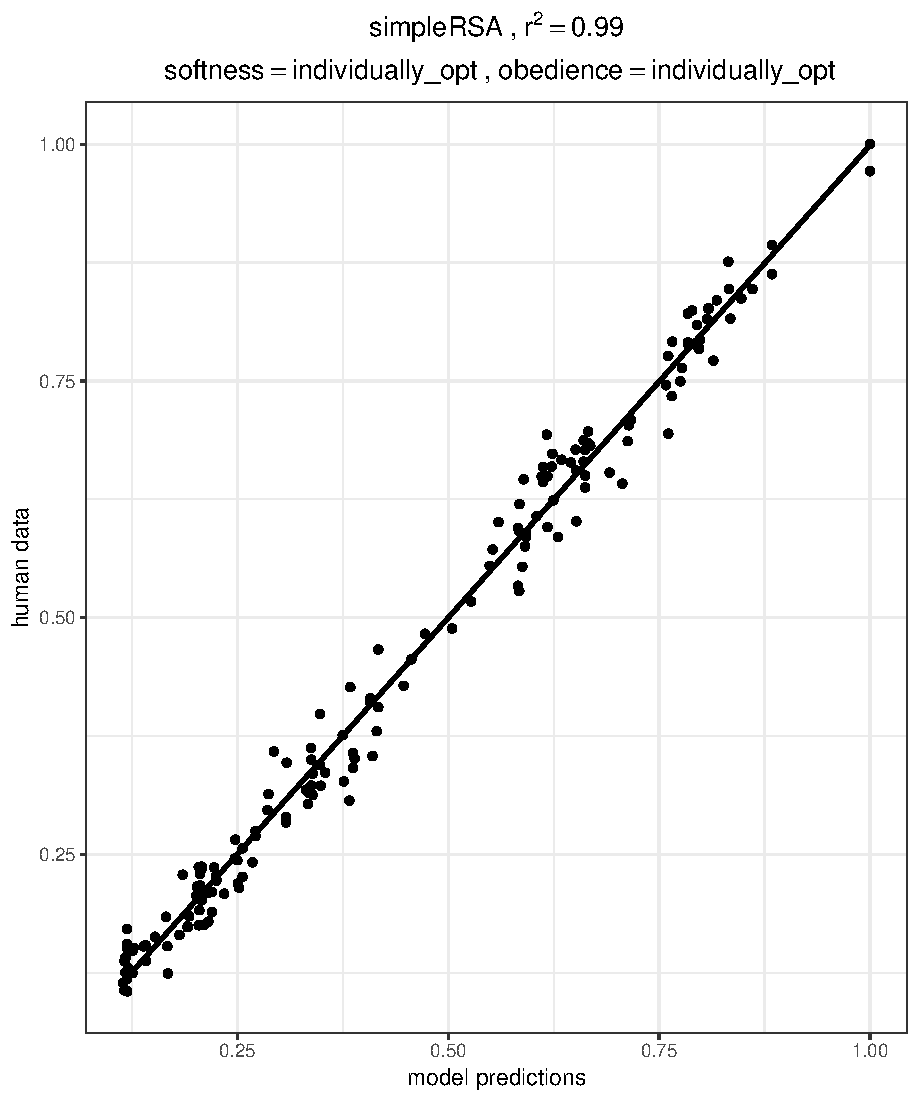
\includegraphics[width=2in]{images/m5.pdf}
	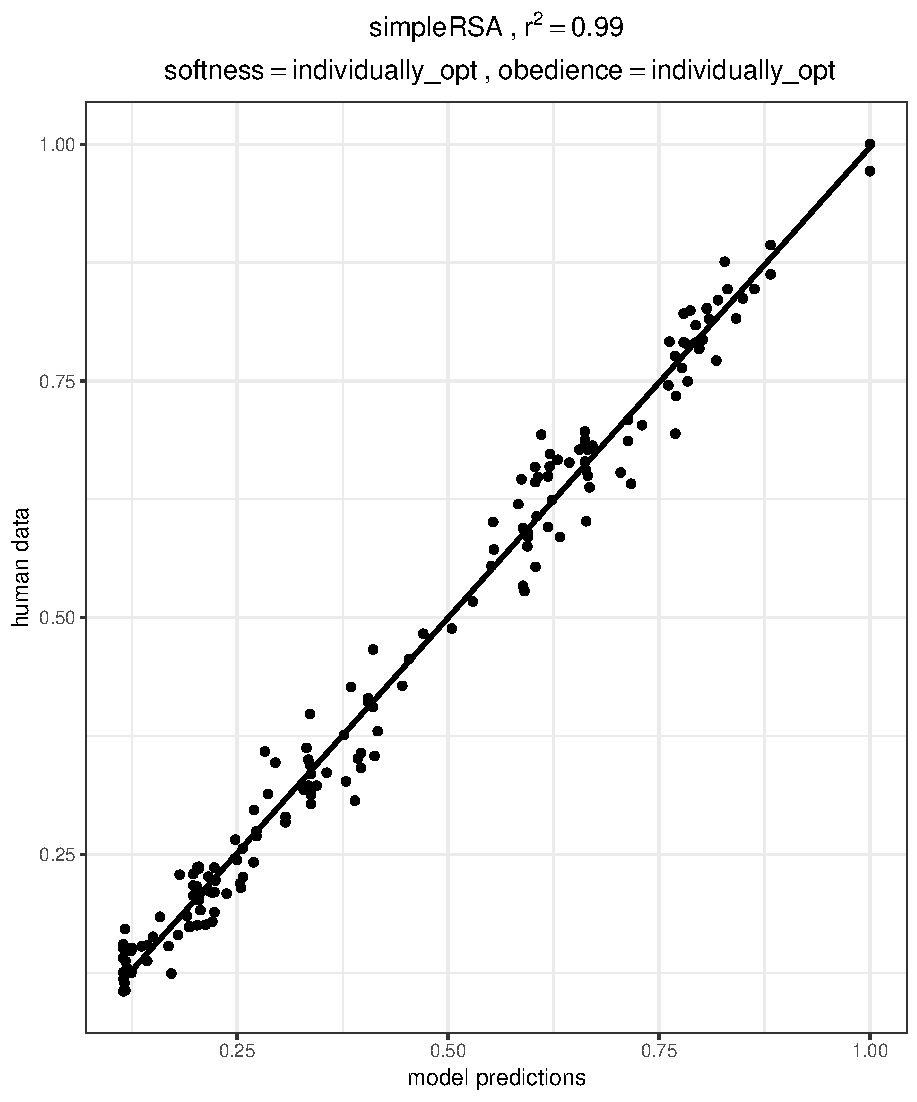
\includegraphics[width=2in]{images/m8.pdf}
	\caption{Average human data from Experiment 1 plotted against the predictions of the individually $\beta$ and $\gamma$-optimized simplified RSA model, non-cross-validated (left panel) $r^{2}=0.99$, 95\% CI [0.98 1.00] and cross-validated (right panel) $r^{2}=0.99$, 95\% CI [0.98 1.01] .}\label{cross-validation}
\end{figure}


Thus, we find strong empirical support for our extended RSA model of preference inference: speakers are indeed able to use listener behavior to arrive at information about their preferences. The question now turns to whether speakers are able to capitalize on this reasoning when it comes to selecting utterances. In other words, are speakers aware that ambiguous language is potentially more informative?

%\FloatBarrier 
% tried to keep figures in relevant sections but it doesn't look too good yet. Maybe when we have final text it will work out

\section{Experiment 2: Choosing utterances}

Our next task is to check the predictions of our strategic utterance selection model: given a set of potential referents, are participants able to reason pragmatically about the utility of ambiguous utterances in informing listener preferences?

\subsection{Participants}

We recruited 90 participants with US IP addresses through Amazon.com's Mechanical Turk crowdsourcing service; participants in Experiment 1 were not eligible to participate in Experiment 2. Participants were compensated for their participation. On the basis of a post-test demographics questionnaire, we again identified  82 participants as native speakers of English; their data were included in the analyses reported below.

\subsection{Design and methods}

Participants encountered a reference game scenario similar to Experiment 1 in which a speaker signals an object to a listener who might have a preference for certain types of objects. However, rather than observing the utterance and referent choice, participants were now tasked with helping the speaker choose an utterance that was ``most likely to reveal the listener's color, shape, or pattern preferences.''

\begin{figure*}[ht]
	\centering
	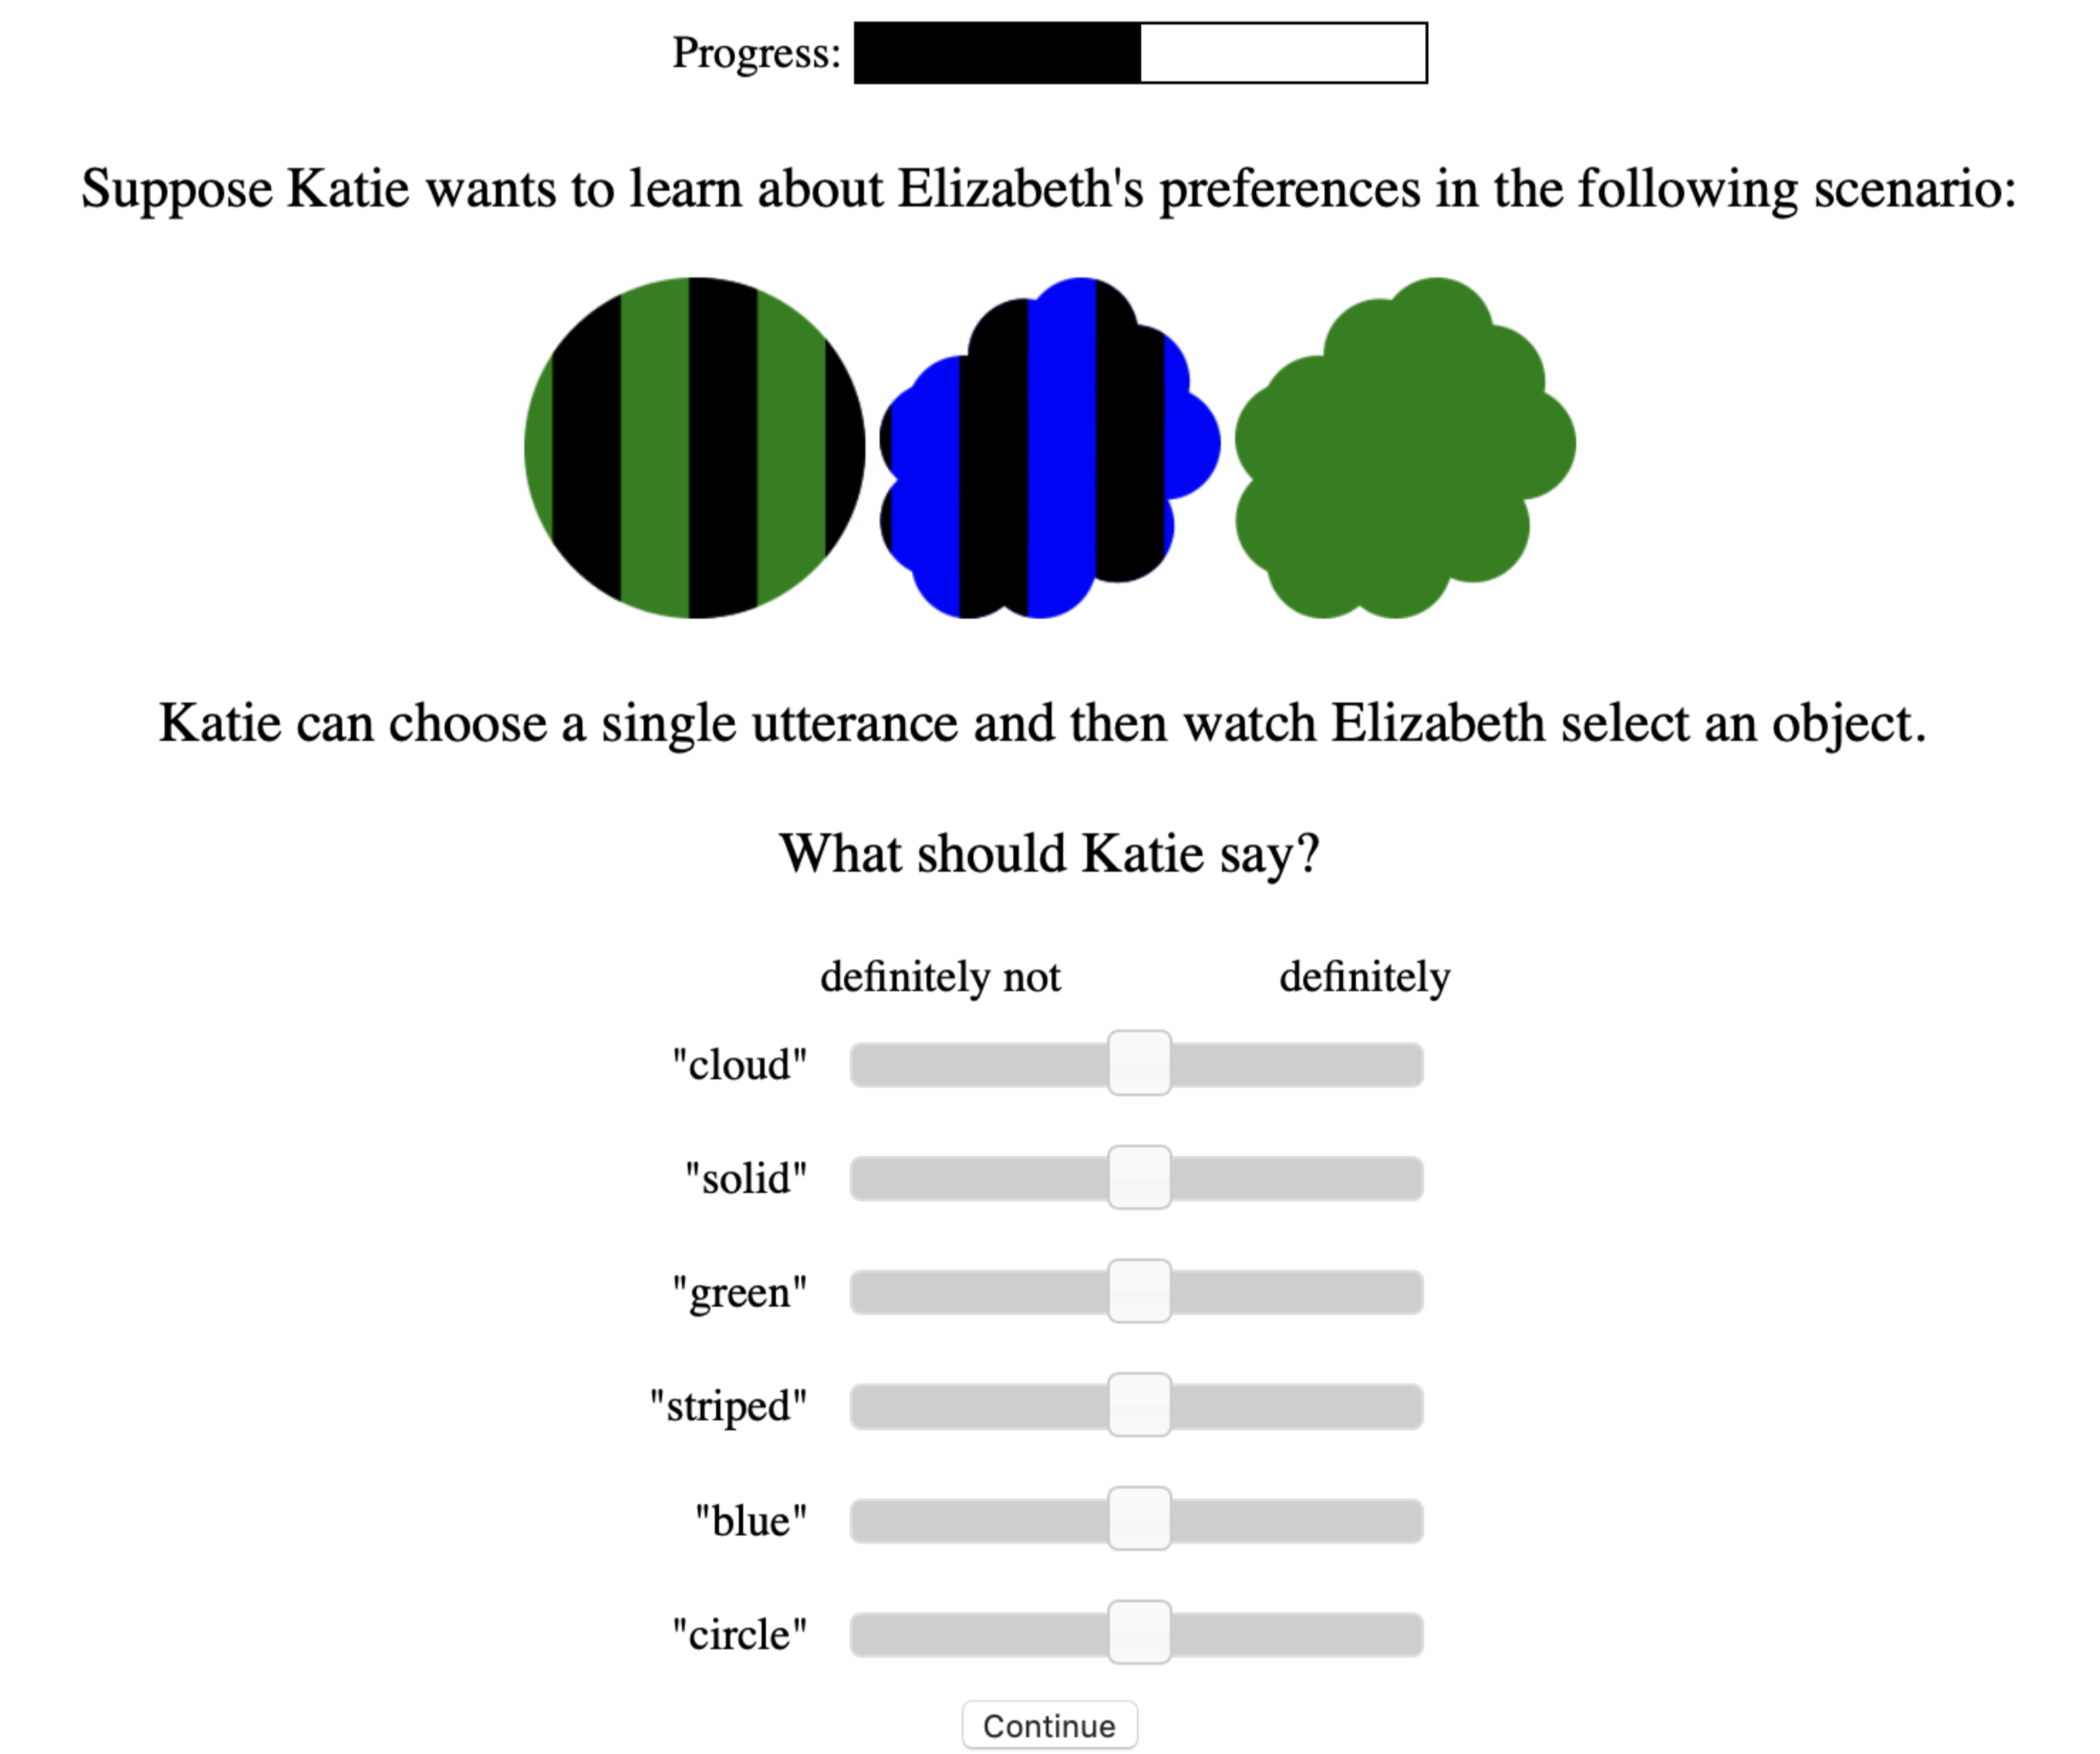
\includegraphics[width=3.5in]{images/utterance-choice-trial.png}
	\caption{A sample trial from \emph{Experiment 2: Choosing utterances}.}\label{exp2-trial}
\end{figure*} 

We used the same sets of objects from Experiment 1, which could vary along three dimensions. Each trial featured a set of three objects, as in Figure \ref{exp2-trial}. After observing the objects, participants adjusted sliders to indicate which single-feature utterance the speaker should choose. Potential utterances corresponded to the features of the objects present; depending on the number of unique features, participants adjusted between three and nine sliders. As with Experiment 1, we averaged the data and the respective model predictions across specific ambiguity classes, which include all scenes that yield identical utterance choice options. 
In this case, $14$ distinct conditions can be identified, with a total of $84$ slider values to set. 
Membership within an ambiguity class is defined by how many objects in a scene share each of the features: shape, pattern and color. If objects share a feature, we also consider whether these objects also share other features. For example, in Figure \ref{exp2-trial}, two green objects differ in shape, making the utterance \textit{green} informative. If, on the other hand, both green objects were clouds, uttering \textit{green} would not let the speaker update their belief about listener's preferences.
In the most extreme case, when all objects share all three features we are dealing with identical objects. In that situation, all utterances are ambiguous since multiple objects can be picked but no utterance allows the speaker to learn anything about the listener since the object choice is uninformative. Another extreme case is a situation when all objects are unique and do not share any features. Then any utterance will only pick 1 object, making learning about preferences impossible.

Participants completed a series of 15 trials. As with Experiment 1, objects were chosen at random, with the constraint that 10 trials were potentially informative with respect to listener preferences (as in Figure \ref{exp2-trial}) and 5 trials were uninformative with respect to listener preferences (e.g., observing a set of three identical objects).



\subsection{Results}


By reasoning the about predictions of $S_2$, we are able to use our extended RSA model to compute the expected most informative utterance with respect to inferring preferences. In other words, $P_b(u)$ calculates the probability that a speaker would choose $u$ for the purpose of inferring preferences in our reference game scenario.

To generate predictions from $P_b(u)$, a total of four free parameters can be identified. 
As with the analysis for Experiment 1, we consider different values for $\alpha$ (i.e., speaker's soft-max factor) and $\gamma$ (i.e., preference softness), and obedience $\beta$. 
We must also set the $\lambda$ parameter, which factors the importance of choosing the expected most informative utterance with respect to the determined KL divergence values.
Note that when allowing negative values for $\lambda$, negated information gain essentially minimizes expected information gain.
Thus, with negative values for $\lambda$, the model favors unambiguous utterances. 
Moreover, when $\lambda=0$, the model collapses to a uniform distribution of utterance choices 
%\gcs{is this true? Will utterances that can describe more objects be preferred?}. Asya: verified with Martin, the description is correct.


%The proper model fit is confirmed when considering the correlation between the participants' data and the model predictions. 

Figure \ref{simple-full-x3} shows the model fits of the unfit full and simple RSA models, with both models failing to predict the human data.

%Figure \ref{exp2-results} plots predictions from the $\lambda$-optimized model, together with the human data. Again, we observe a strong positive correlation between the human judgments and model predictions ($r^2 = 0.91, p < 0.001$). In other words, we find evidence in support of the idea that speakers reason pragmatically about the relative informativity of ambiguous language.

\begin{figure}[ht]
	\centering
	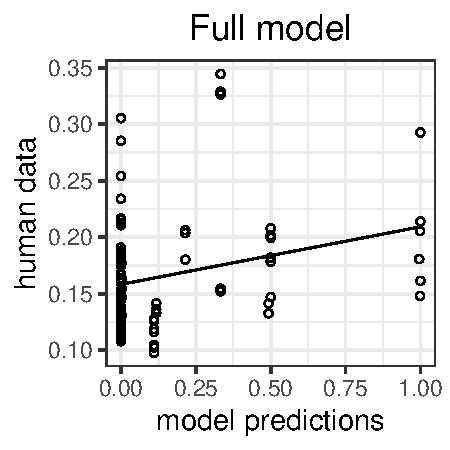
\includegraphics[width=2in]{images/x3_m1.pdf}
	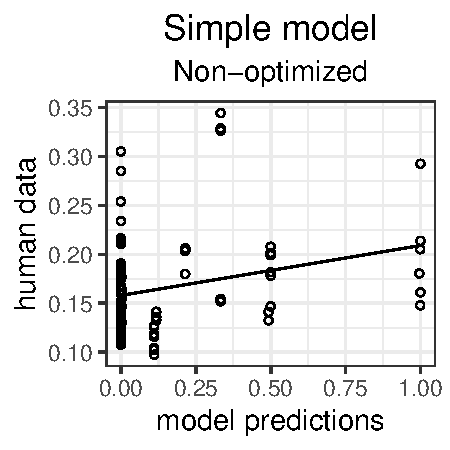
\includegraphics[width=2in]{images/x3_m7.pdf}
	\caption{Average human data from Experiment 2 plotted against the predictions of the parameter-free RSA model; both models $r^{2}=0.07$, 95\% CI [0.01.23].}\label{simple-full-x3}
\end{figure}

% I recorded the same number of conditions as in Experiment 1. I think Experiment 2 used the same ambiguity code.

%The results for the base model yielded an average KL divergence value of $5.415$ (median=$3.997$), while the $\lambda$-optimized model yielded a mean KL divergence of $3.774$ (median=$2.108$).
%Again determining $G^2$ to enable a Chi-square test for significant model differences in fitting the data, the difference between the base model and one-parameter model (factored by $2*15=30$) of $49.23$ (median difference of $56.67$) is highly significant, indicating that the one-parameter model fits the data much better than a uniform base model. 
% Note: these interesting observations may not be mentioned _ I leave them in for now because the discussion can relate to them 

To fit model parameters, we again optimized values with respect to KL divergence estimates between the participant data and the model predictions---in this case for utterance preference distributions.  We compared three individually-optimized models to determine which model provides the best linear fit to the data. All the models have similar levels of complexity with either softness $\gamma$, obedience $\beta$, or KL-value factor $\lambda$ being optimized. The results indicate that we get the best fit by optimizing the KL-factor $\lambda$ ($r^{2}=0.91$; cross-validated optimization $r^{2}=0.89$), with other models capturing less variance in the data: obedience ($r^{2}=0.80$), softness of preferences ($r^{2}=0.81$). Two- and three-parameter optimization were unstable due to parameter interactions, therefore we do not report the results for those models here.

Unlike for Experiment 1, where even the parameter-free models ensured a good linear fit to the data, optimization produces a large effect on the model predictions in Experiment 2. We illustrate this effect with the predictions of the model for the sample trial (Figure \ref{exp2-trial}). Figure \ref{barplot_x3} shows that in a situation with a  striped green circle, a blue striped cloud, and a solid green  cloud, uttering things like \textit{cloud}, \textit{striped}, or \textit{green} and then observing the listener pick an referent could let the speaker learn something about the listener's preferences. For example, \textit{green} picks out two objects: a striped green circle and a solid green cloud; after saying ``green'', the speaker could learn whether the listener prefers striped things over solid things, or circles over clouds.

\begin{figure}[ht!]
	\centering
	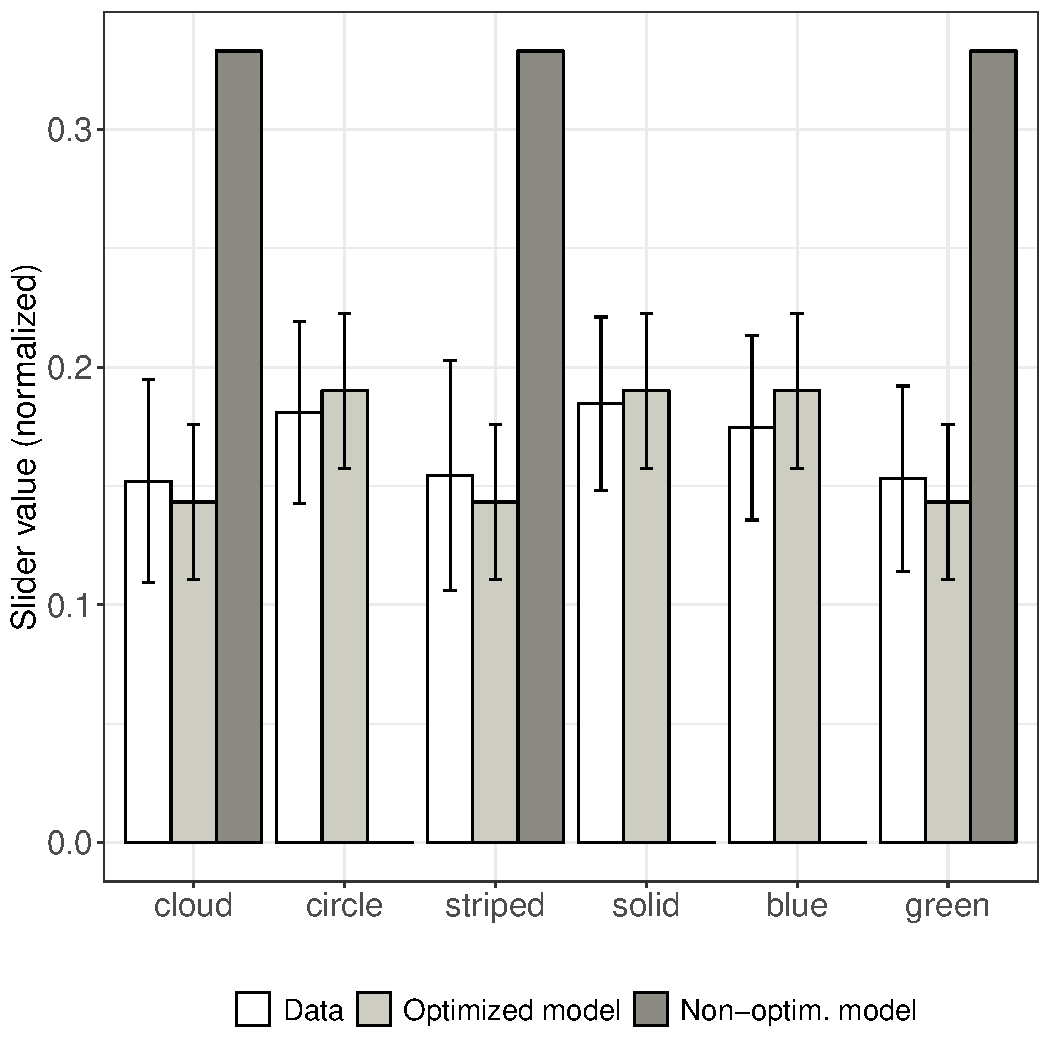
\includegraphics[width=2.5in]{images/barplot_x3.pdf}
	\caption{Model predictions and human data for one of the classes of stimuli \emph{Experiment 2: Picking utterances}.}\label{barplot_x3}
\end{figure}

% Note: I did check it - there are indeed 14. 5+5+6+7+6+6+7+3+4+5+6+7+8+9
%After matching the respective actual feature values with the utterance choice relevant within the respectively-binned conditions, we again computed averages over utterance preference values for the respectively-binned trials across participants and across respective model predictions \gcs{this is awfully hard to follow}. Asya: decided to remove this part, reordering can just as well stay behind the scenes.


In Figure \ref{kl-factor} we compare a $\lambda$-optimized model (right panel) to a uniform base model (left panel) that assigns equal probability to each utterance available for a particular context.
 %\gcs{how is this model defined?} Asya: it really is a model that takes the probability of 1 and distributes it evenly between all possible utterances.
 A model with the $\lambda$ parameter optimized at the individual level fits the data better than a uniform model  (Likelihood ratio test: $G = 268.87, df = 82, p <0.01$). 
\begin{figure}[ht]
	\centering
	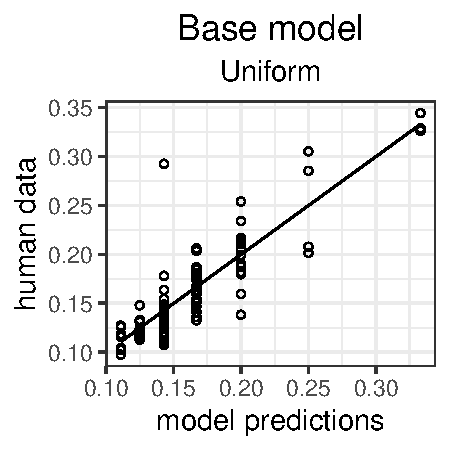
\includegraphics[width=2in]{images/x3_m20.pdf}
	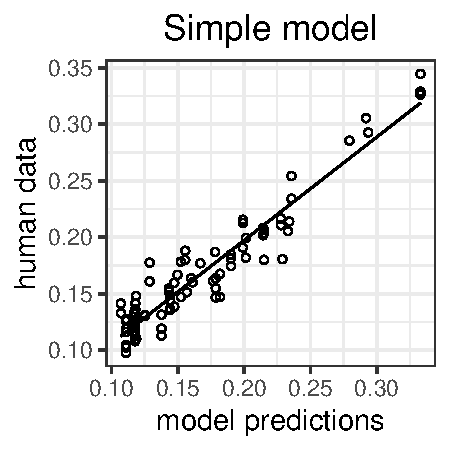
\includegraphics[width=2in]{images/x3_m11.pdf}
	\caption{Average human data from Experiment 2 plotted against the predictions of the uniform and simple RSA models; uniform model  $r^{2}=0.75$, 95\% CI [0.65 0.84], KL-factor optimized  $r^{2}=0.91$, 95\% CI [0.92 1.06]]. }\label{kl-factor}
\end{figure}

We were able to distinguish three groups of participants on the basis of the fitted parameter values of $\lambda$. 
The first was a ``lazy worker'' group of $18$ participants whose fitted $\lambda$ values were close to zero (i.e.,  $-.02 < \lambda<.02$).
The second group of $32$ participants yielded more negative values (i.e., $-7.13<\lambda<-.02$), indicating that a significant number of participants preferred to systematically choose unambiguous utterances. 
The third group of again $32$ participants yielded more positive values (i.e., $.02<\lambda<.54$), indicating that these participants indeed chose the most ambiguous utterance in a strategic manner. 


\section{General discussion}

We have found strong support for our model of inferring priors on the basis of ambiguous language.
% \gcs{we might want to talk about this as ``priors'' in the introduction as well} Asya: added a new section to the Intro
The results of Experiment 1 demonstrate that na\"ive speakers are able to reason pragmatically about \emph{why} listeners may take the actions they do, and the success of our computational model in predicting the observed behavior offers an articulated hypothesis about \emph{how} this reasoning proceeds: when speakers are aware of the ambiguity in their utterances, observing how listeners resolve that ambiguity provides clues to the preferences listeners use when doing so.
The results of Experiment 2 demonstrate that at least some speakers are able to capitalize on this reasoning to strategically select ambiguous utterances that are most likely to inform their understanding of the preferences of their listeners.

Taken together, the results of our experiments and the success of our model in predicting those results indicate that humans are aware of the fact that by observing responses to ambiguous utterances, information about the listener's prior preferences can be inferred. 
Used in this way to inform preferences, ambiguous utterances are closely related to questions, which may ask directly about the  relevant preferences. 
However, ambiguous language provides a ready alternative to asking directly. In normal conversations, a speaker might favor the indirect route afforded by ambiguous utterances, given considerations of politeness and possibly also in an effort to keep the conversation open, in that the conversation partner can choose to disambiguate the ambiguous utterance or, alternatively, choose to continue in a different direction or even to change topic.


We note that the analyzed preference prior, viewed from a broader perspective, can be closely related to a part of the predictive mind of the listener and the speaker \cite{Butz:2016,Butz:2017}. 
When interpreting an utterance -- in our case opening up a set of choices -- the listener's mind infers the current choices and integrates them with the preference priors, implicitly anticipating possible choice consequences.
Moreover, the expected information gain term -- computing the utterance choice of the speaker -- can be equated with the computation of socially-motivated active inference \cite{Butz:2017a,Friston:2015}.
It causes the model to strive for an anticipated epistemic value that quantifies the expected information gain about the assumed preference priors of the listener, that is, expected social information gain. 


In general, predictive states of mind about others do not only include considerations of the preferences of others, but generally may concern all imaginable knowledge, opinions, beliefs, current train of thought considerations, and preferences of the listener.
Moreover, during a conversation, the involved ``social'' priors will dynamically develop depending on the internal predictive models and the generated utterances, actions, and responses of the speaker and listener. 
The prior dynamically depend on the privileged grounds of the conversational partners, and also on the common ground in which the conversation unfolds.
In that sense, ambiguous utterances are one device for projecting parts of each others' privileged grounds into the common ground. 


%Moreover, there 
%in conversation the priors dynamically unfold according to beliefs and preferences about the world and speakers
%twin anecdote, politeness (why not ask directly?)
%is ambiguity a feature that evolved under pressure from these considerations (i.e., informing preferences), or did ambiguity predate these considerations and speakers merely figured out clever ways of capitalizing on it---a lemonade-out-of-lemons scenario?

\bibliographystyle{apacite}
\setlength{\bibleftmargin}{.125in}
\setlength{\bibindent}{-\bibleftmargin}

\bibliography{prior-inference}

\end{document}

